\documentclass[varwidth=true, border=2pt]{standalone}

\usepackage{tkz-fct}
\usetikzlibrary{arrows}

\begin{document}
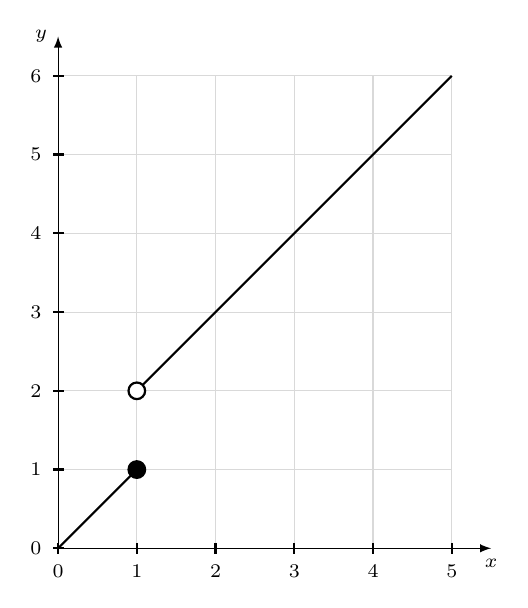
\begin{tikzpicture}
       \tkzInit [xmin=0,xmax=5,ymin=0,ymax=6]
        \begin{scriptsize}
            \tkzGrid[color = gray!30!white]
            \tkzAxeXY
        \end{scriptsize}
        \draw[thick] (0,0) -- (1,1);
        \draw[thick] (1,2) -- (5,6);
        \draw[thick,fill=black] (1,1) circle (3pt);
        \draw[thick,fill=white] (1,2) circle (3pt);
\end{tikzpicture}
\end{document}
